\documentclass[11pt]{article}
\usepackage{a4wide}
\usepackage{times}
\usepackage[french]{babel}
\usepackage[T1]{fontenc} 
\usepackage[utf8]{inputenc}
\usepackage{url}

\usepackage{eurosym}
\usepackage{amssymb}
\usepackage{xcolor}
\newcommand{\mynote}[3][black]{\textcolor{#1}{\fbox{\bfseries\sffamily\scriptsize{#2}}
{\small$\blacktriangleright$\textsf{\emph{#3}}$\blacktriangleleft$}}}
\newcommand{\pem}[1]{} %{\mynote[cyan]{Pierre-Etienne}{#1}}
\newcommand{\ld}[1]{\mynote[magenta]{Laurence}{#1}}
\newcommand{\TODO}[1]{\mynote[red]{TODO}{#1}}
\newcommand{\TOREMOVE}[1]{\mynote[cyan]{REMOVE}{#1}}
%\newcommand{\TODO}[1]{}
\newcommand{\silent}[1]{}
\newcommand{\gpl}[0]{génie de la programmation et du logiciel}
\newcommand{\eg}[0]{\emph{e.g.},~}
\newcommand{\ie}[0]{\emph{i.e.},~}
\newcommand{\etal}[0]{\emph{et al.}~}
\newcommand{\wrt}[0]{\emph{w.r.t.}~}
\newcommand{\cf}[0]{cf.~}
\newcommand{\defi}[1]{\emph{(défi p.\pageref{#1}, \cite{#1})}}

\usepackage{pdfpages}


\title{GdR Génie de la Programmation et du Logiciel\\ 
Défis 2030? 2026?}
\author{Mireille Blay-Fornarino, Catherine Dubois, Pierre-Etienne Moreau\\
\\
%%\textbf{DRAFT}
}
\begin{document}
\maketitle

\section{Introduction}

Le manifeste rédigé par une partie de la communauté du GDR GPL commence par ces mots : \emph{Le contraste est saisissant entre, d’un côté, l’omniprésence de l’informatique dans notre
société et la facilité avec laquelle on peut écrire un petit programme, et d’un autre côté, la difficulté extraordinaire de garantir la correction, la fiabilité, les performances ou encore
l’évolutivité d’un logiciel complexe comme on en rencontre aujourd’hui dans tous les pans
de notre société : télécoms, aérospatiale, automobile mais aussi finance, santé,
administration, etc}\cite{Manifeste}.
Dans le même temps, l'Association nationale néerlandaise pour le génie logiciel publiait également un manifeste \cite{Nederland2019} qui reprenait le même argumentaire, mais le complétait à peu près en ces mots:  \emph{Bien que les logiciels aient un impact sur chacun de nous tout et partout, l'effort nécessaire pour rendre ces logiciels fiables, maintenables et utilisables sur de plus longues périodes est régulièrement sous-estimé, tant par les développeurs que par leurs responsables. En conséquence, nous voyons tous les jours des articles sur des bogues logiciels coûteux et des projets de développement de logiciels qui dépassent le budget ou qui échouent\footnote{Despite the fact that software impacts everyone everywhere, the effort that is needed to make this software reliable,
maintainable and usable for longer periods is routinely underestimated, both by developers and their managers. As a result,
we see news items every day about expensive software bugs and over-the-budget or failed software development projects\cite{Nederland2019}.}.}


Le Génie de la Programmation et du Logiciel est au c{\oe}ur de l'activité
informatique. Les concepts, méthodes et les outils de conception et de
validation de logiciels constituent les éléments manipulés par les
informaticiens pour maîtriser et automatiser les problèmes qui leur sont
soumis. Avec l'omniprésence de l'informatique dans notre vie que ce soit en termes
d'informatique embarquée, d'intelligence ambiante, d'extension du web au niveau
de la planète, d'intégration dans les objets du quotidien, ou encore avec le
développement de grandes infrastructures de calcul ou de traitement de grandes
masses de données, de nouvelles questions de recherche sont posées.
De nouveaux paradigmes, de nouveaux langages, de nouvelles approches de
modélisation, de vérification, de tests et de nouveaux outils dans le domaine
de la programmation et du logiciel devraient voir le jour dans les 5 à 10 ans à
venir, que ce soit pour faciliter la vie des concepteurs de logiciels, pour
modéliser et fiabiliser les logiciels ou encore pour devancer l'évolution
technologique, mais également pour prendre en compte de nouveaux enjeux de
société tels que le développement durable, les économies d'énergie ou la maîtrise des systèmes intégrant de l'intelligence artificielle.

Au sein du Groupement de Recherche du CNRS sur le Génie de la Programmation et du Logiciel (GDR GPL), les équipes de recherche en France sur ces thématiques ont en décembre 2019, mis en exergue les défis auxquels elles s'intéressent. Dans cet article, nous en proposons une synthèse, non exhaustive, à destination de lecteurs non nécessairement experts du domaine. Les aspects recherche nécessitant des connaissances expertes sont décrits dans les documents joints ci-après.


\TODO{PLAN ET ORGANISATION La confiance est un élément clef...

}




\section{Fiabilité des logiciels}
La fiabilité d'un logiciel exprime la probabilité que celui-ci rende bien le service attendu. Elle se décline ainsi sur différentes dimensions dont la conformité aux objectifs, la sûreté de fonctionnement, la sécurité, les performances,l'efficacité énergétique, ... 
C'est un des défis majeurs d'un monde numérique, maintes fois mis en exergue par nombre de chercheurs dont Gérard Berry \cite{berry} et Xavier Leroy\cite{leroy}. Si des avancées majeures ont été obtenues par des technologies de preuves, de vérification, de tests, de surveillances, il reste de nombreux défis à résoudre pour rendre les systèmes logiciels plus sûrs et améliorer notre confiance dans ces systèmes. 
Les chercheurs en GPL aspirent ainsi à une continuité entre l'expression d'un problème, la mise en oeuvre et la maintenance de la solution logicielle, continuité qui devrait permettre de tracer, vérifier, faire évoluer les applications avec une plus grande fiabilité (cf.~\ref{ss:fiabilite:continuite}). Celle-ci implique de maîtriser non seulement le lien entre la spécification et sa traduction en programmes, mais également l'exécution du programme, qui dépend des compilateurs utilisés et de l'environnement dans lequel il s'exécute (cf.~\ref{ss:fiabilite:execution}).
Ces recherches relèvent simultanément des champs théoriques et pratiques.

\TODO{FINIR d'Introduire le plan de cette partie :  }

\subsection{De l'idée à la mise en oeuvre\label{ss:fiabilite:continuite}} 
La construction d'un système est aujourd'hui l'affaire de nombreux acteurs des développeurs aux utilisateurs eux-même, mais également d'exigences multiples (\eg énergie, sécurité, performance) voir contradictoires. La composition de ces différentes préoccupations est alors une tâche d'une très grande complexité qui revêt différents aspects, dont la qualification des services (\eg Qualité de service, d'expérience), la mise en place de modèles de coordination \defi{reconfiguration}.



Depuis plusieurs années, les montées en abstraction portées par l'ingénierie des modèles et des langages ont permis de renforcer la fiabilité des logiciels "par construction" en garantissant le respect des propriétés définies à plus haut niveau. Les chercheurs en GPL aspirent ainsi à une continuité entre l'expression d'un problème et les exigences associées, la mise en oeuvre et la maintenance de la solution logicielle.
Néanmoins pour appréhender la fiabilité d'une application dans sa globalité il est nécessaire d'avoir les moyens de décrire avec suffisamment de détails les propriétés spécifiques attendues et de raisonner en intégrant de nombreux paradigmes dont l’exécution du programme par un ou plusieurs processeurs et avec des données ou dans des conditions potentiellement imprévues et ceci dès sa conception \cite{reconfiguration, compilation}. 
C'est particulièrement le cas pour les systèmes logiciels qui dépendent d'impératifs du monde réel, tels que les systèmes cyber-physiques. On constate des besoins similaires pour les systèmes intégrant de l'apprentissage automatique qui restent difficiles à tester au sens du génie logiciel et pour lesquels les notions de qualités logicielles restent à définir~\cite{IA}.  La fiabilité des  applications émergentes intégrant  systèmes cyber-physiques et intelligence artificielle, dont par exemple les voitures autonomes, soulèvent ainsi un grand nombre de questions de recherches tant du point de vue de l'expression des propriétés recherchées que des outils permettant de les vérifier~\cite{emergents}.

Comme nous l'avons vu précédemment, la construction d'un système est aujourd'hui l'affaire de nombreux acteurs des développeurs aux utilisateurs eux-même, mais également d'exigences multiples (\eg énergie, sécurité, performance) voir contradictoires. La composition de ces différentes préoccupations est alors une tâche d'une très grande complexité qui revêt différents aspects, dont la qualification des services (\eg Qualité de service, d'expérience), la mise en place de modèles de coordination \defi{reconfiguration}.
la conception de langages et d'outils à haut niveau d'abstraction pour l'expression de la qualité de service (QoS) et de la qualité d'expérience (QoE) du point de vue de l'utilisateur final, et la traduction associée en un processus de reconfiguration coordonné et sûr, piloté par les différents aspects de la QoS/QoE.



\TODO{sécurité by design ... et le défi sécurité??? pas vu ??}

\subsection{Du programme à son exécution\label{ss:fiabilite:execution}}
Les preuves peuvent s'appliquer à différents niveaux de description d'un programme, de sa spécification à son exécution. Cependant la traçabilité entre ces différents niveaux est très difficile à établir. 
Ainsi même si les compilateurs ne sont jamais que du code permettant de transformer des programmes en d'autres programmes, il reste très difficile de les vérifier. En effet, un des intérêt des compilateurs est d'optimiser les exécutions, en s'adaptant aux environnements d'exécution, sans exiger du programmeur de s'intéresser à ces aspects.  Si des travaux tels que CompCert, un compilateur C optimisant, permettent de garantir mathématiquement la même sémantique entre la source et le programme assembleur généré, de nombreux verrous doivent encore être levés, dont la gestion de la concurrence sur les processus et les données, la capacité des codes exécutés ou interprétés à supporter des environnements d'exécution difficiles\todo{??}, à se protéger d'attaques matérielles, …
~\defi{Monniaux}.
Cette problématique rejoint la question de la production de logiciels éco-responsables qui utilisent efficacement les ressources en fonction des contextes d'exécution\cite{vert}. 

\subsection{Des outils pour élaborer la confiance}
Un des points difficiles dans l'ensemble des éléments relevés précédemment est la construction des éléments de confiance eux-même. Il est indispensable de disposer d'outils qui permettent d'élaborer ces preuves complexes avec plus de facilité, nous retrouvons cette dimension dans \cite{Monniaux, reconfiguration}.  

\subsection{Informatique de confiance}
Avec quels éléments de preuve, est-il raisonnable d'avoir confiance dans un système? Comment justifier qu'un système est bien construit? Ces questions vont au-delà de la preuve ou du test d'un système. Elles nous ramènent à  la problématique de l'accessibilité au raisonnement suivi pour donner confiance dans un système que ce soit ou non dans un objectif de certification \defi{argumentation}. 
Elles abordent sous un nouvel angle, des verrous tels que la 
complémentarité entre preuves, tests et simulations, les relations entre les artefacts logiciels et les exigences, entre la construction des éléments de preuve et la construction du système, etc. 

\section{Production, Maintenance et évolution efficiente des logiciels}
\TODO{NTRODUIRE cette partie :  Nous faisons le choix ici de présenter simulténément la production de logiciels et la maintenance}

Un grand nombre des systèmes logiciels sont aujourd'hui distribués, concurrents, de très grande taille et appelés à s'adapter automatiquement aux changements de contexte d'exécution (\eg les systèmes Cloud, Fog, Edge et cyber-physiques). 
Dans le même temps, la production de nouveaux composants intégrés à ces systèmes, les évolutions des interactions entre ces composants, des réseaux et des composants eux-même, dirigées par des contextes d'exploitation changeant et des impératifs de rapidité, ont conduit à accélérer les changements de méthodes et pratiques de production et maintenance des logiciels.   Au delà d'une question d'agilité, il s'agit de se donner les moyens de produire des logiciels que nous maîtrisons, y cmpris dans le temps \cf. \ref{ss:maintenance:debugger}, qui répondent et s'adaptent à nos besoins \cf 2 \ref{ss:maintenance:reconfiguration}, et dans lesquels nous avons confiance,

Nous faisons ici le choix de présenter quelques unes des questions de recherche posées par l'explosion en besoin de production et maintenance des logiciels.


\subsection{Reconfiguration dynamique et automatique des systèmes \label{ss:maintenance:reconfiguration}}
Comme la structure des systèmes peut être utilisée en cours d'exécution pour découvrir des services ou adapter des composants, une reconfiguration dynamique correcte devient un aspect important de l'exécution du système. La conception d'outils formels intégrés de niveau d'abstraction supérieur pour aider à la conception d'une reconfiguration sûre, tolérante aux pannes et efficace des logiciels distribués est alors essentielle \defi{reconfiguration}

Consommation des logiciels....




\subsection{Logiciels durables}
Les logiciels qui nous entourent doivent répondre aux besoins spécifiques de chacun, y compris dans des contextes métiers particuliers. Le problème est bien connu et les réponses apportées varient des architectures logicielles (en ce moment les micro services) au langages dédiés, en utilisant différentes techniques dont l'ingénierie des modèles. \ref{coevolution}

\subsection{Maintenir, une exigence d'abstractions \label{ss:maintenance:abstractions}}
L'expression des systèmes et solutions en utilisant les abstractions adaptées en fonction des objectifs 
est exploitée en infomatique depuis au moins Grace Murray Hopper \cite{DBLP:journals/sigcse/Gurer02} pour améliorer l'efficience de la production d'applications que ce soit par exemple dans les formalismes de construction de preuves, de langages dédiés, d'administrations, d'environnement de production de logiciels, etc.

Ces dernières années, différents outils ont été élaborés pour permettre aux utilisateurs de définir leurs  propres abstractions afin de construire des langages dédiés pour augmenter leur productivité, des environnements .....
Ces abstractions sont alors exploitées par composition, génération et/ou configuration de code. La question de la maintenance est alors éminemment complexe puisqu'il s'agit de s'adapter en même temps à l'évolution des concepts, aux mécanismes qui les exploitent, aux cibles. On parle alors de co-évolutions. Si le problème est connu, les avancées en GL et les données accumulées dans ces processus devraient permettre de proposer des solutions plus automatiques, rapides et efficaces\defi{coevolution}, et de les prendre en compte dans l'étape difficile de recherche de défauts \defi{debuggers}.

Dans le contexte de la Combinatoire certifiée, définir les théories logiques et des langages de spécification et de programmation adaptés aux objets de la combinatoire reste un défi \defi{combinatoire}.




\subsection{Maintenir, une exigence de première classe \label{ss:maintenance:debugger}}
Face à la complexité des logiciels, malgré les grandes évolutions méthodologiques incluant le test et la preuve, il reste difficile aujourd'hui de réparer et adapter les logiciels alors même que quelques fois la simple reproduction d'un comportement est difficile. La construction des logiciels et les 
logiciels eux-même utilisent aujourd'hui des paradigmes évolués (e.g. concurrence des tâches, présences de modèles  non déterministes dans les architectures, communications par des composants tiers, masses des codes générés). 

Mais appréhender la recherche de défauts comme une discipline à part entière, à prendre en compte comme un élément essentiel aux développements même des nouveaux supports de production d'application est un défi pour une gestion efficace des logiciels \defi{debugger}.

\subsubsection{La maintenance face aux générateurs de code \label{ss:maintenance:debugger}}
Comme nous en avons discuté précédemment, les logiciels sont souvent produits par génération de code. La question de la maintenance est alors éminemment complexe impliquant de modifier les générateurs de code qu'il s'agisse d'atteindre de nouvelles cibles ou d'adapter les générateurs aux évolutions des abstractions de plus haut niveaux. Comment appréhender ces co-évolutions ? Comment concevoir les générateurs de codes pour qu'ils supportent celles-ci ? les données existent… 
Face aux masses de codes ainsi produites, les outils aujourd'hui ne sont pas adaptés qu'il s'agisse de les évaluer \defi{coevolution} ou de les prendre en compte dans l'étape difficile de recherche de défauts \defi{debugger}


\TODO{Vers plus de fiabilité sur les résultats de recherche en génie Logiciel}

\section{Conclusion A REVOIR}
Nous utilisons nos techniques parce que nous avons besoin d'outil et que ces outils sont eux même du logiciel

\bibliographystyle{plain}
\bibliography{gdrGPLDefis}
\section*{Défis}
\begin{enumerate}
\item \defi{combinatoire}
\item \defi{vert}
\item \defi{GLE}
\item \defi{debuggers}
\item \defi{securite}
\item \defi{coevolution}
\item \defi{compilation}
\item \defi{reconfiguration}
\item \defi{argumentation}
\item \defi{IA}
\item \defi{Monniaux}
\item \defi{formelle}
\end{enumerate}
\section{Conclusion}


\label{vert}
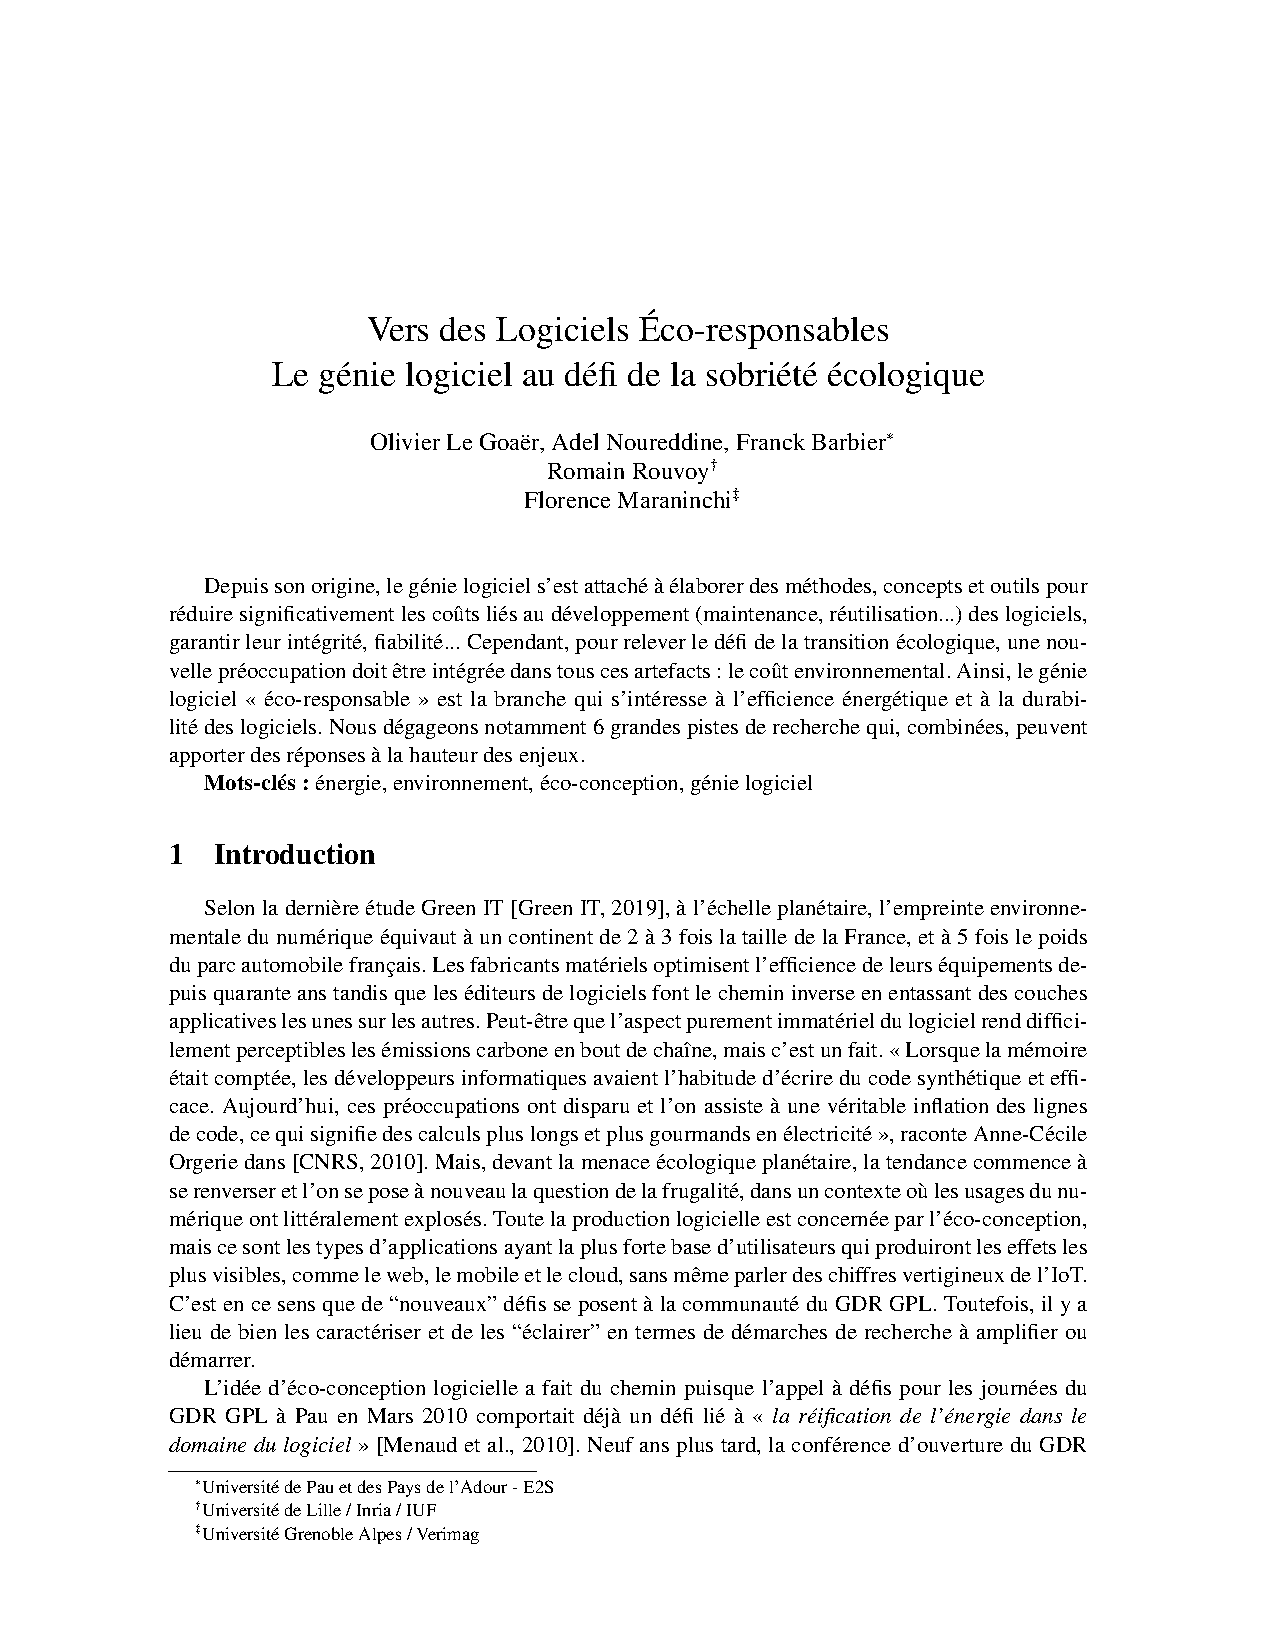
\includepdf[pages=-,pagecommand={\thispagestyle{plain}}]{Defis/logiciels_verts.pdf}

\label{combinatoire}
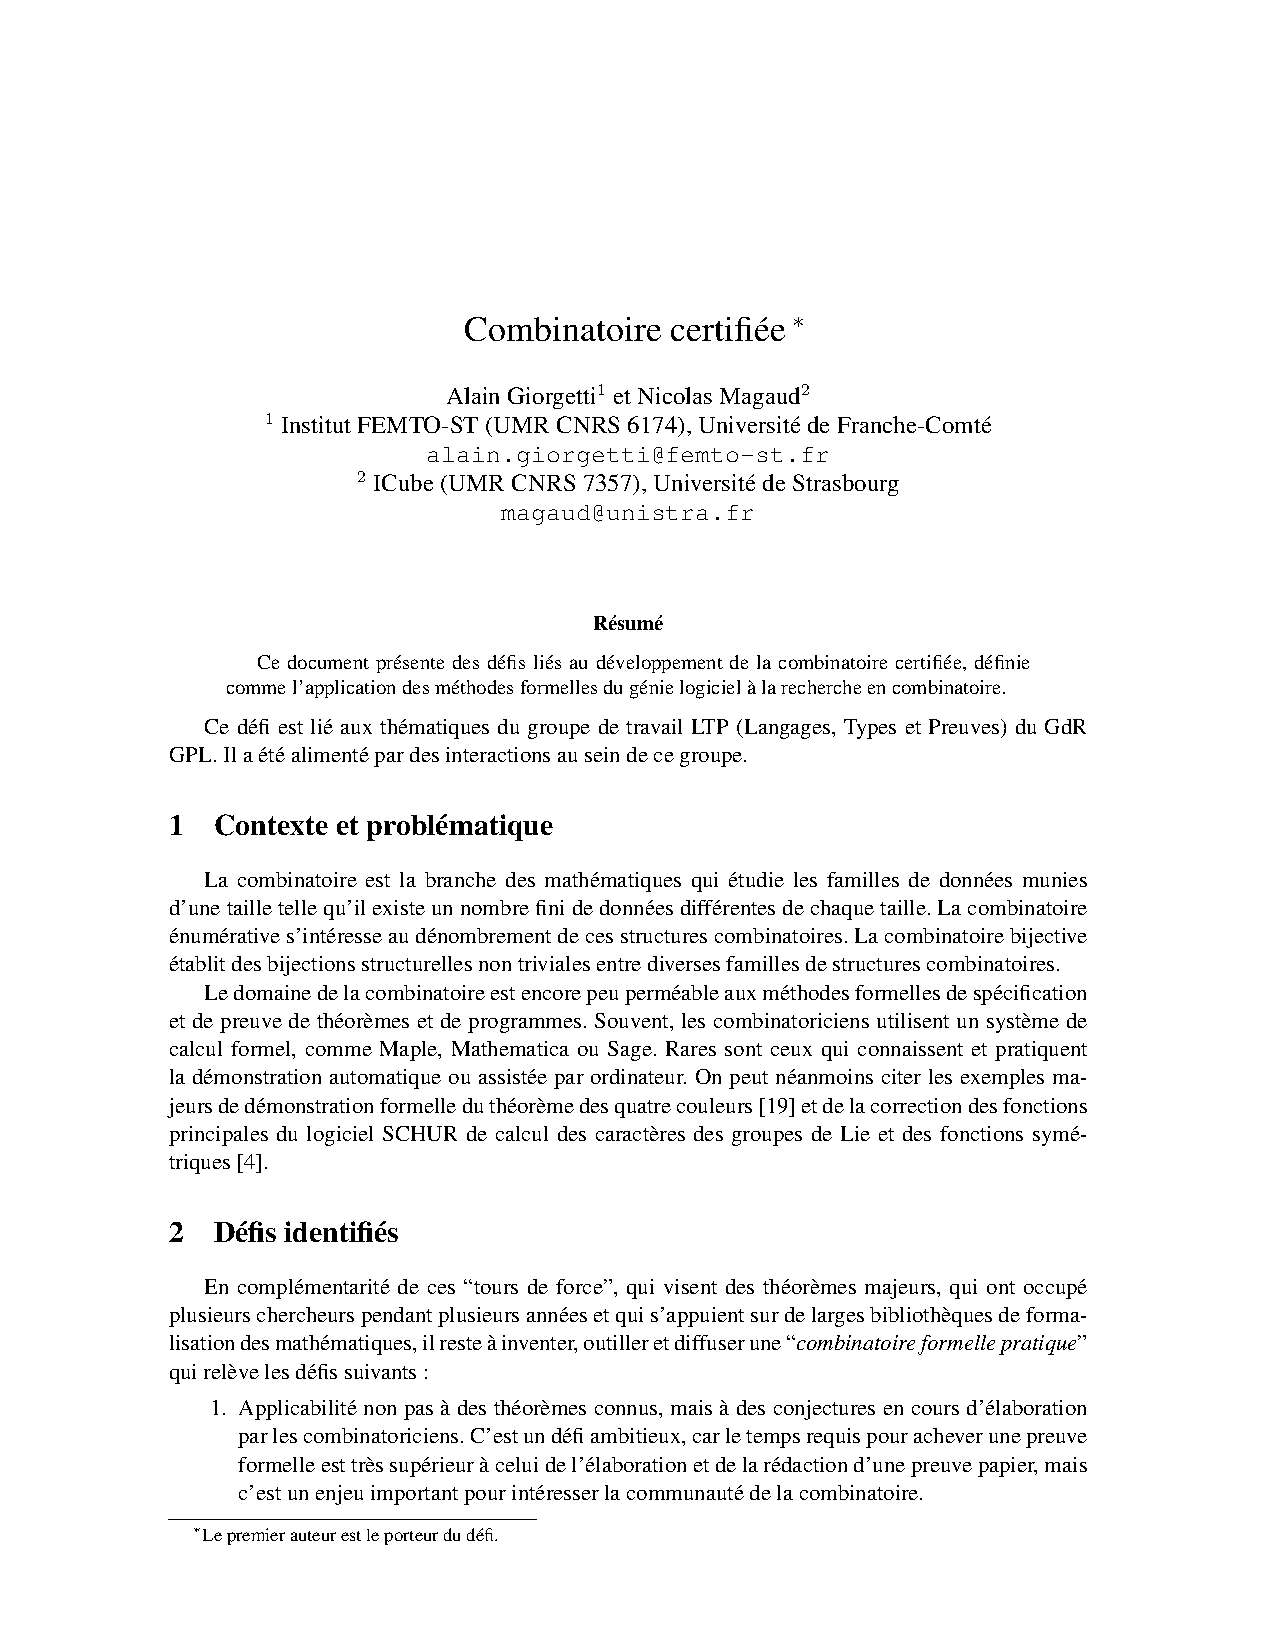
\includepdf[pages=-,pagecommand={\thispagestyle{plain}}]{Defis/combinatoire_certifiee.pdf}

\label{formelle}
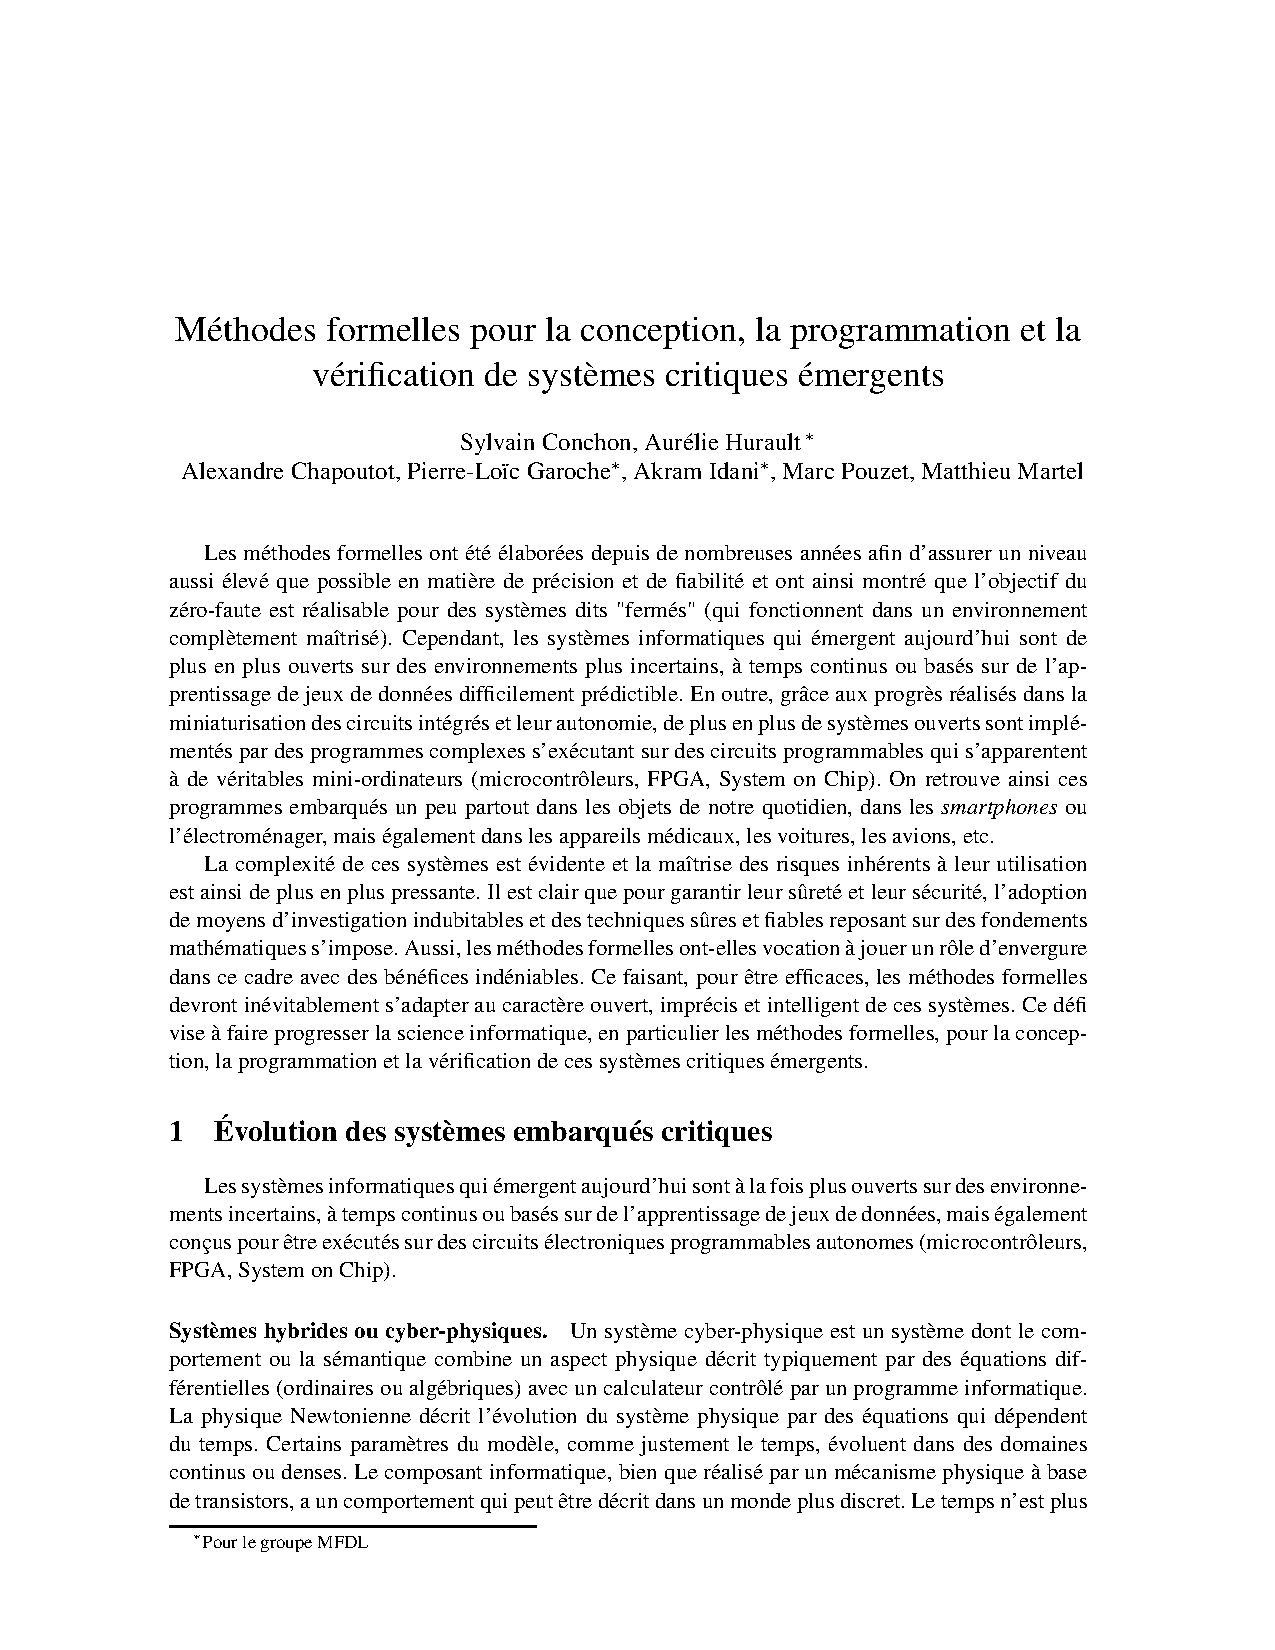
\includepdf[pages=-,pagecommand={\thispagestyle{plain}}]{Defis/FM_systemes_emergents.pdf}







\label{argumentation}
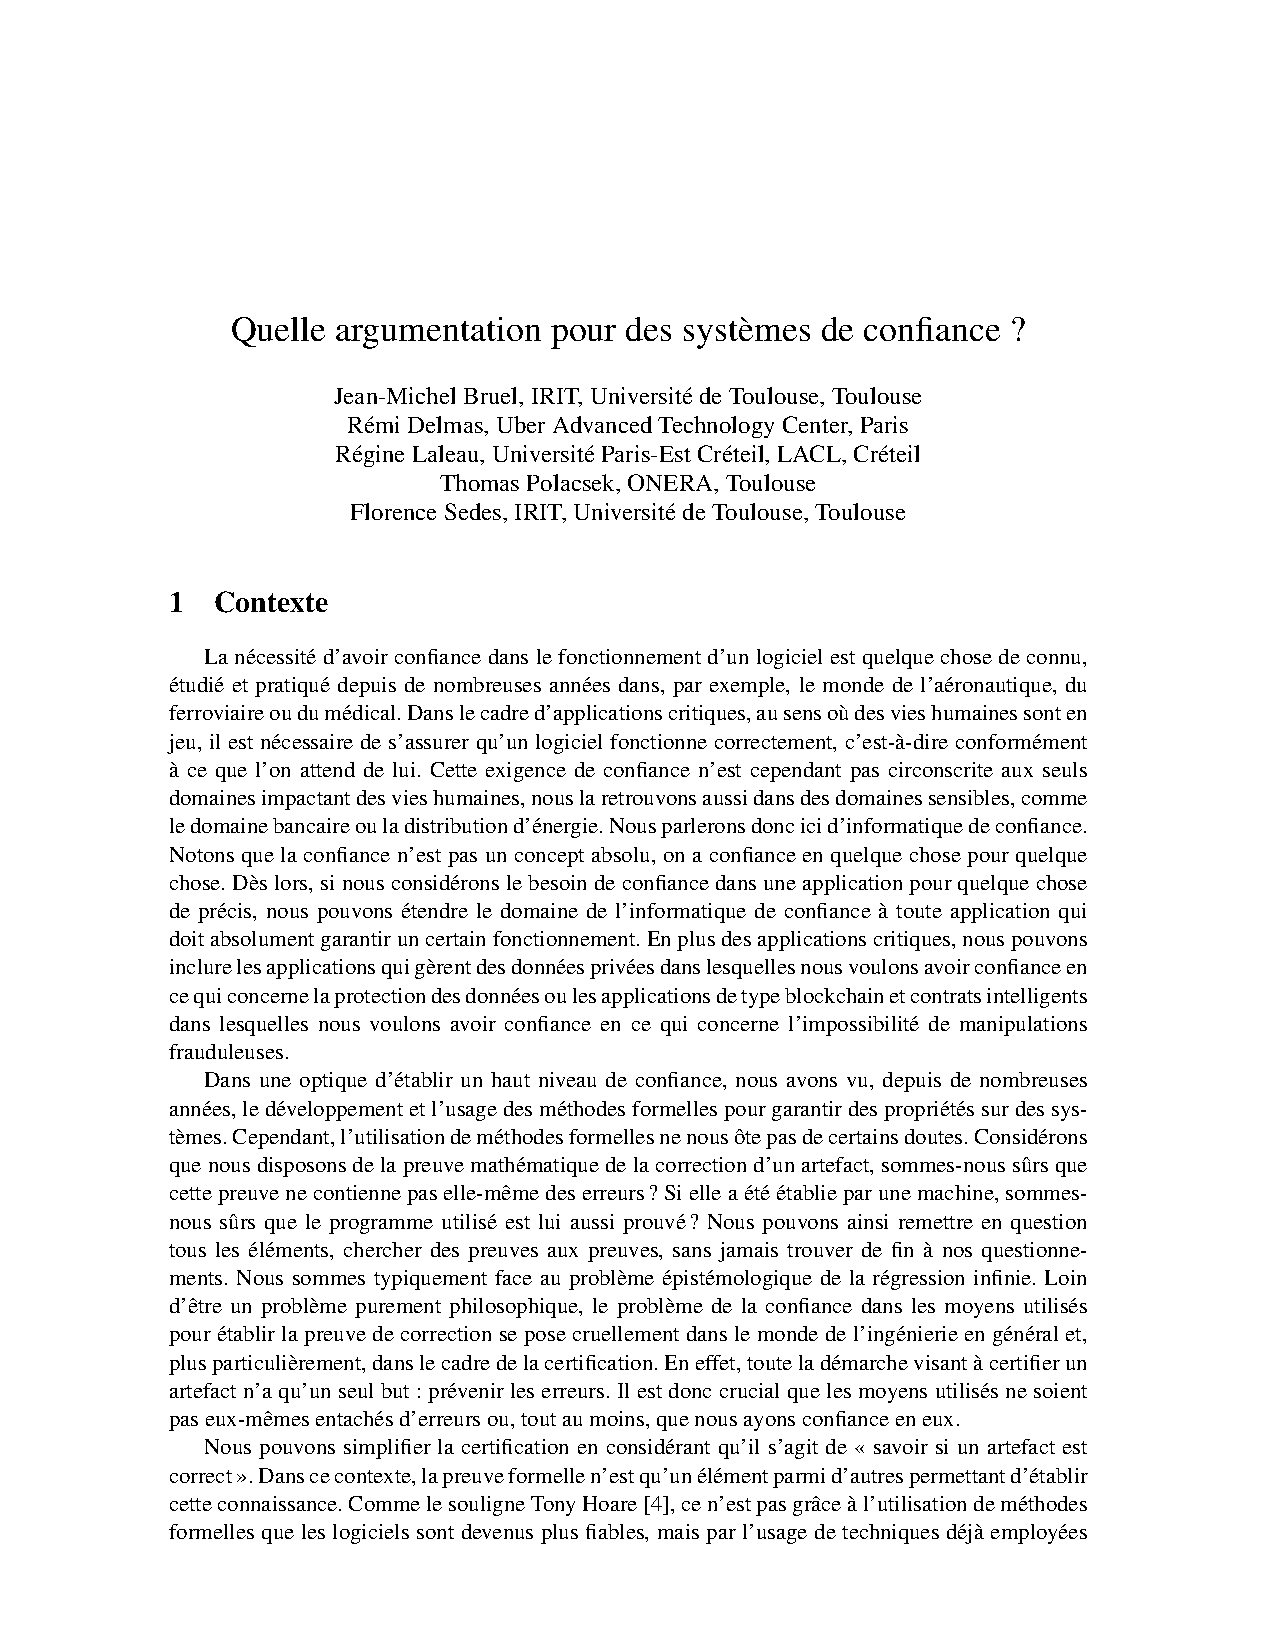
\includepdf[pages=-,pagecommand={\thispagestyle{plain}}]{Defis/argumentation_pour_des_systemes_de_confiance.pdf}

\label{Monniaux}
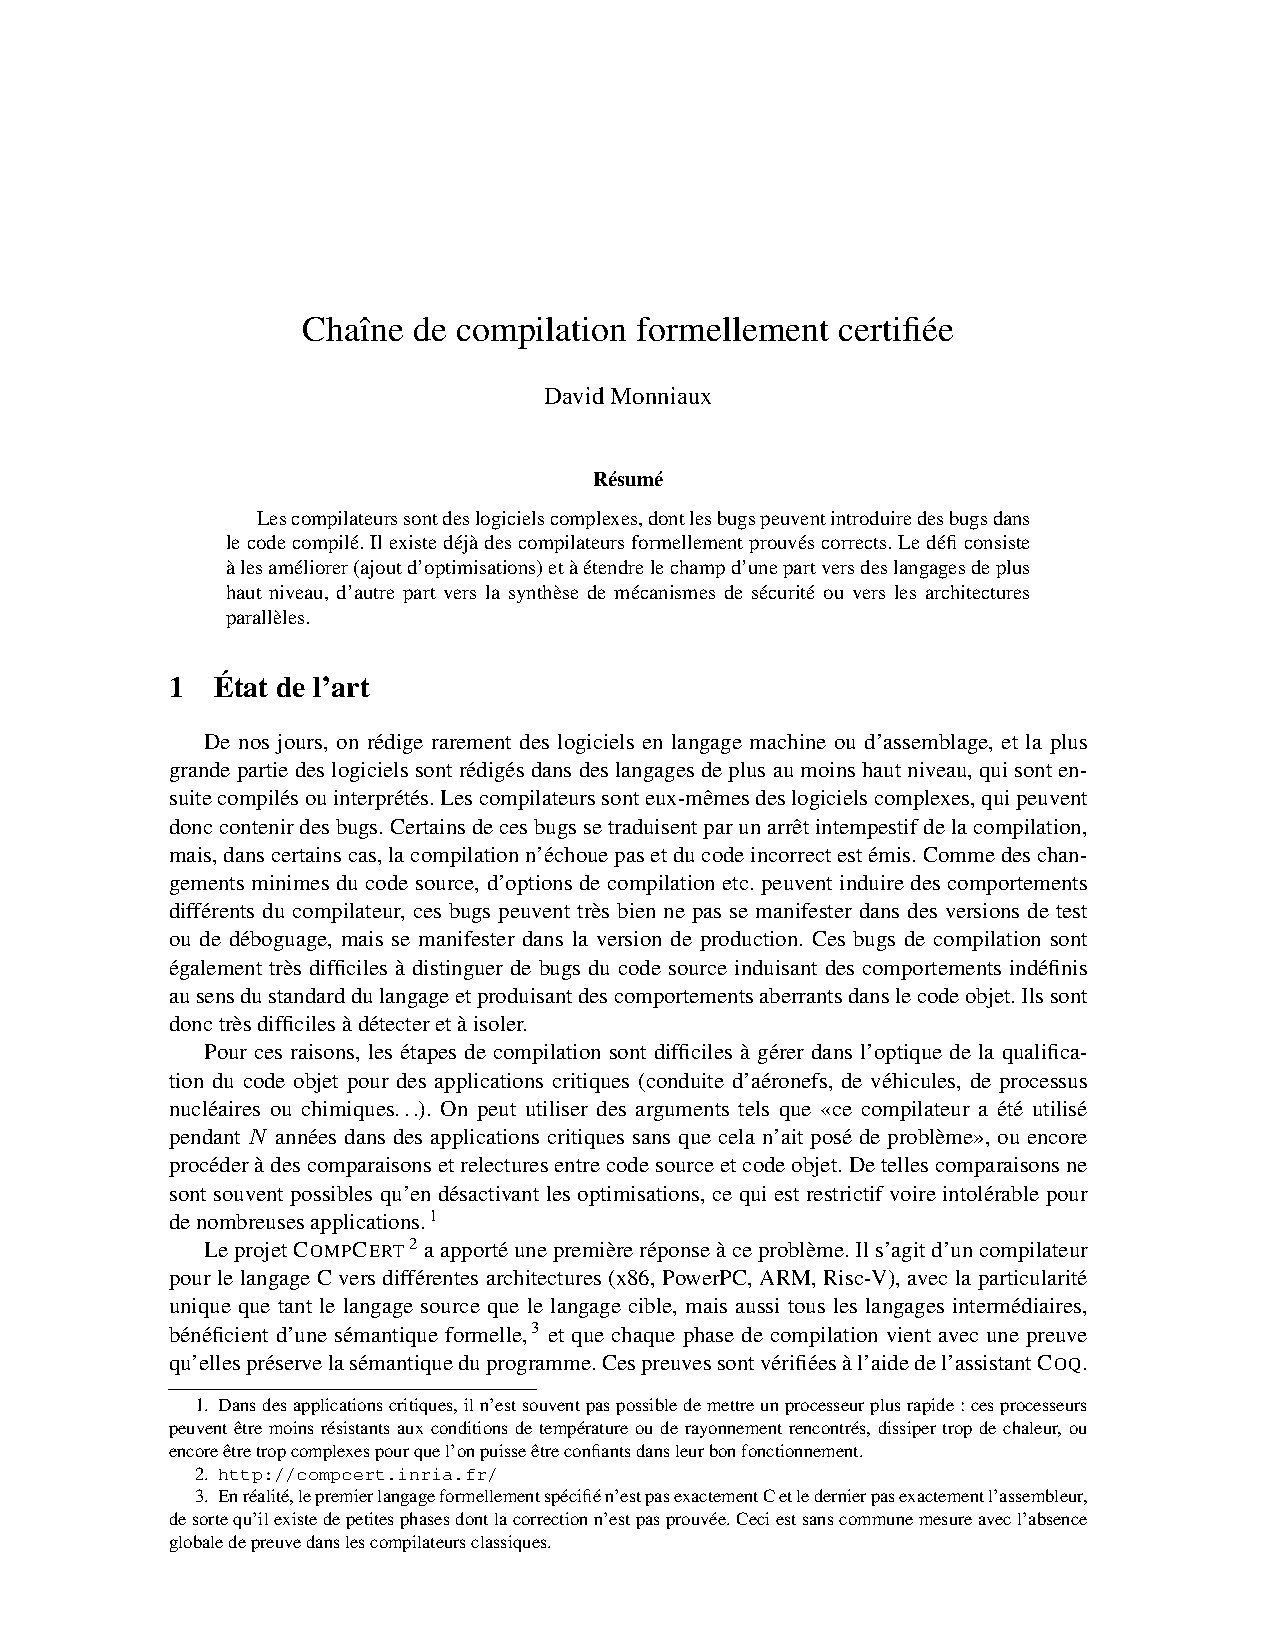
\includepdf[pages=-,pagecommand={\thispagestyle{plain}}]{Defis/chaine_compilation_certifiee.pdf}

\label{coevolution}
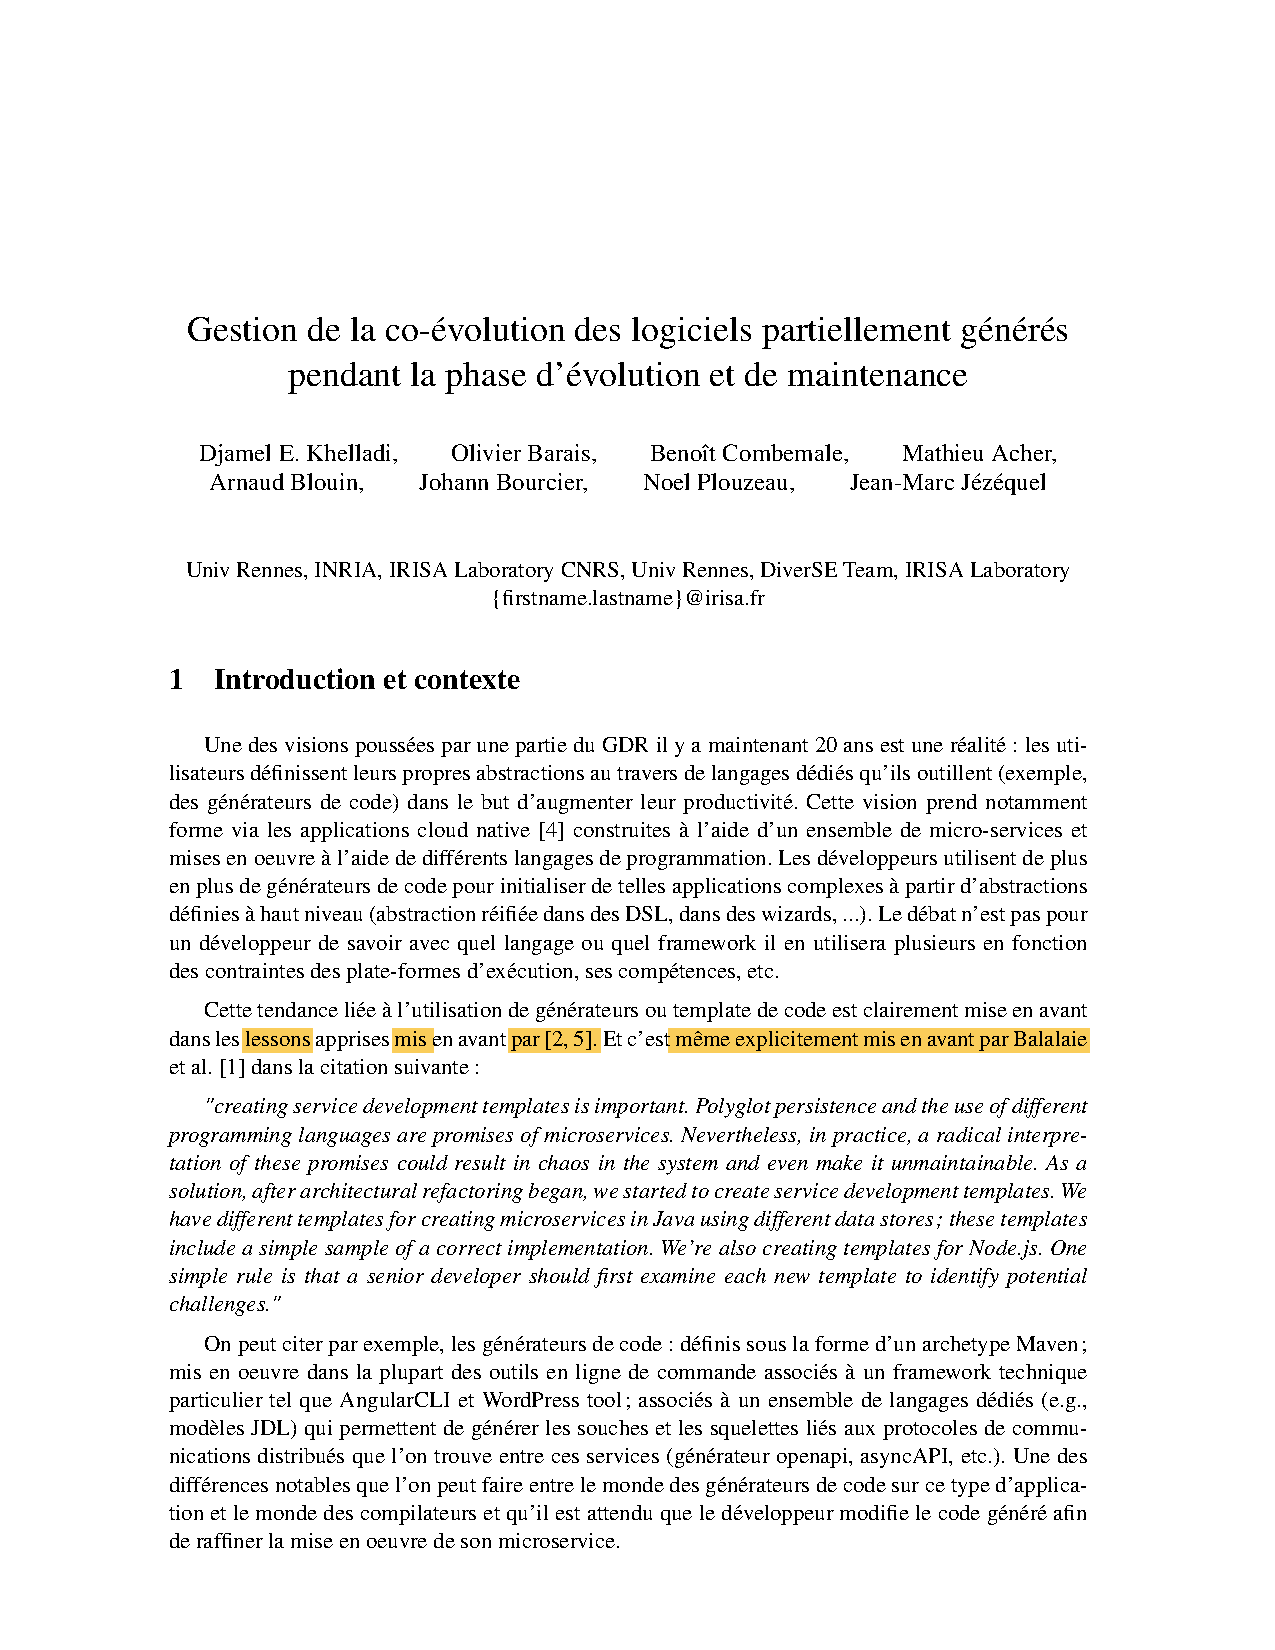
\includepdf[pages=-,pagecommand={\thispagestyle{plain}}]{Defis/co-evolution_des_logiciels.pdf}

\label{compilation}
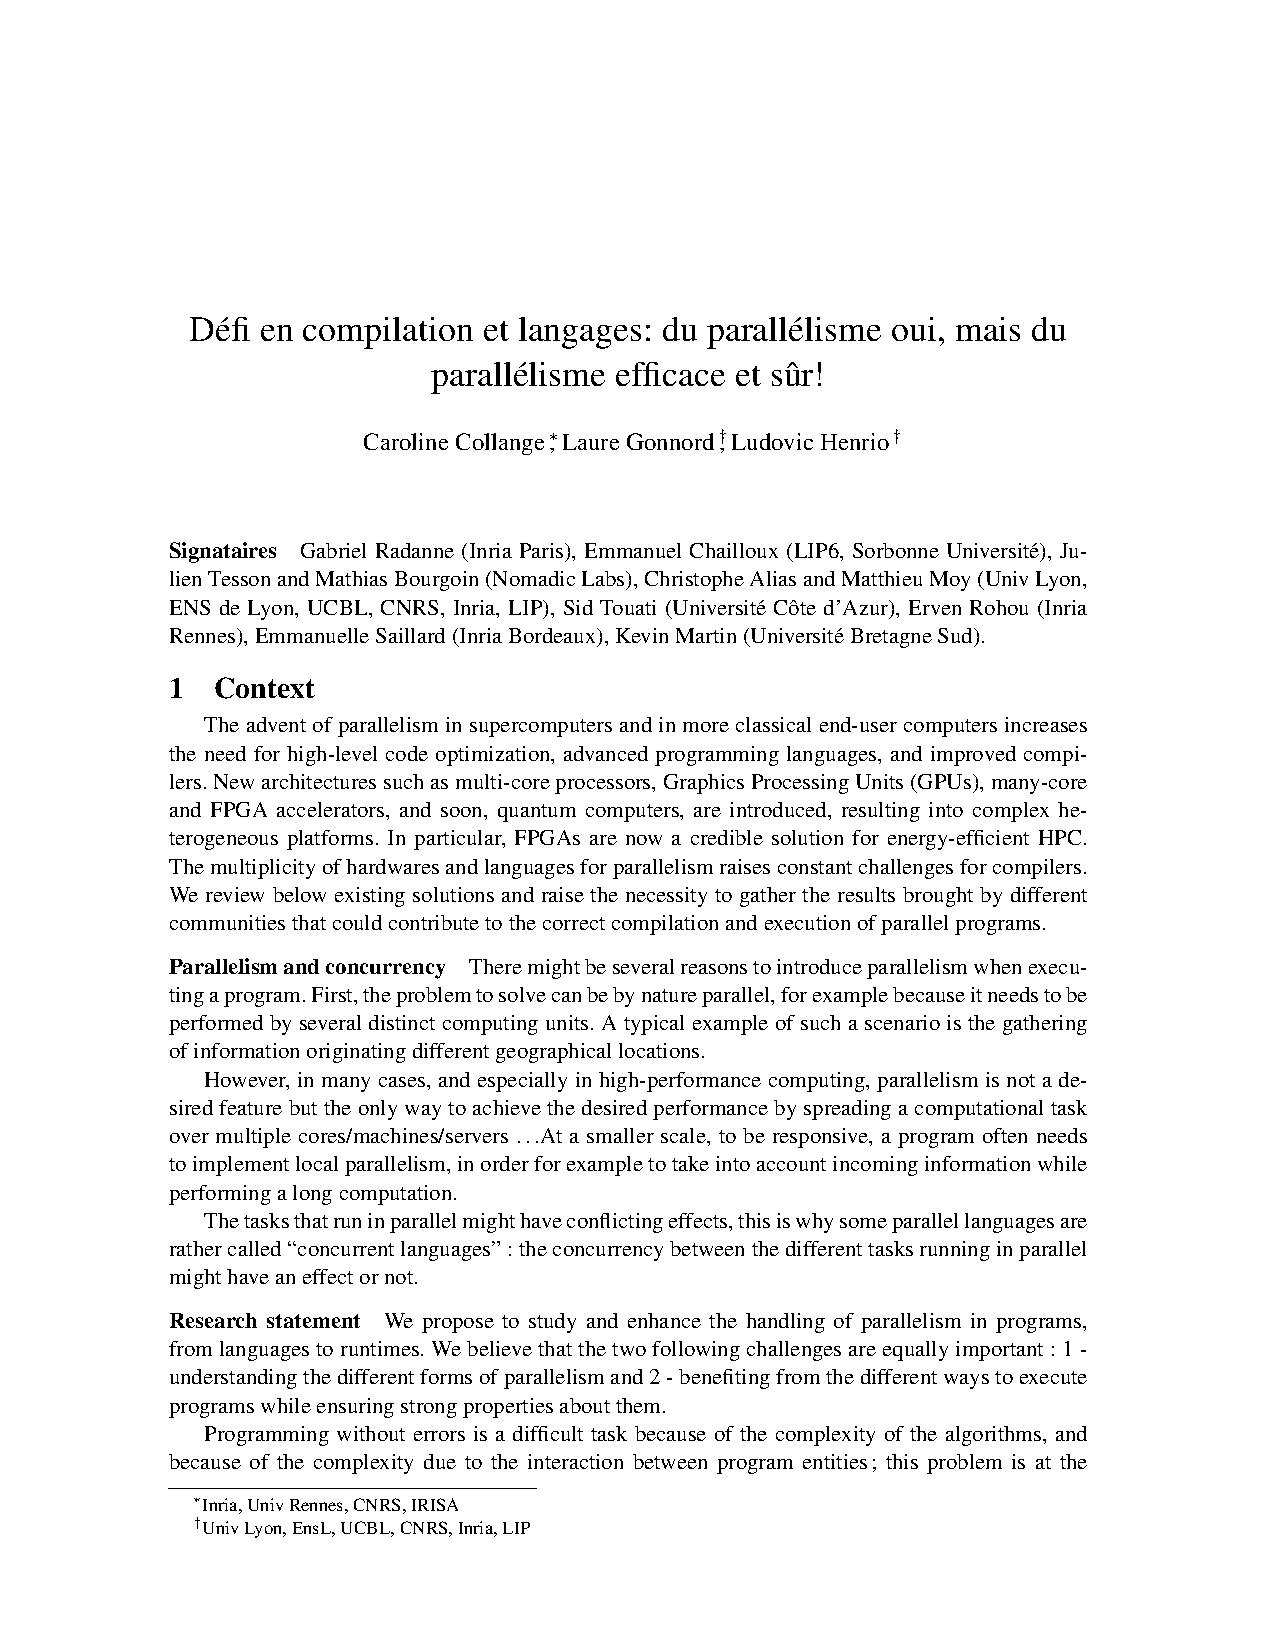
\includepdf[pages=-,pagecommand={\thispagestyle{plain}}]{Defis/Compilation_et_langages.pdf}

\label{IA}
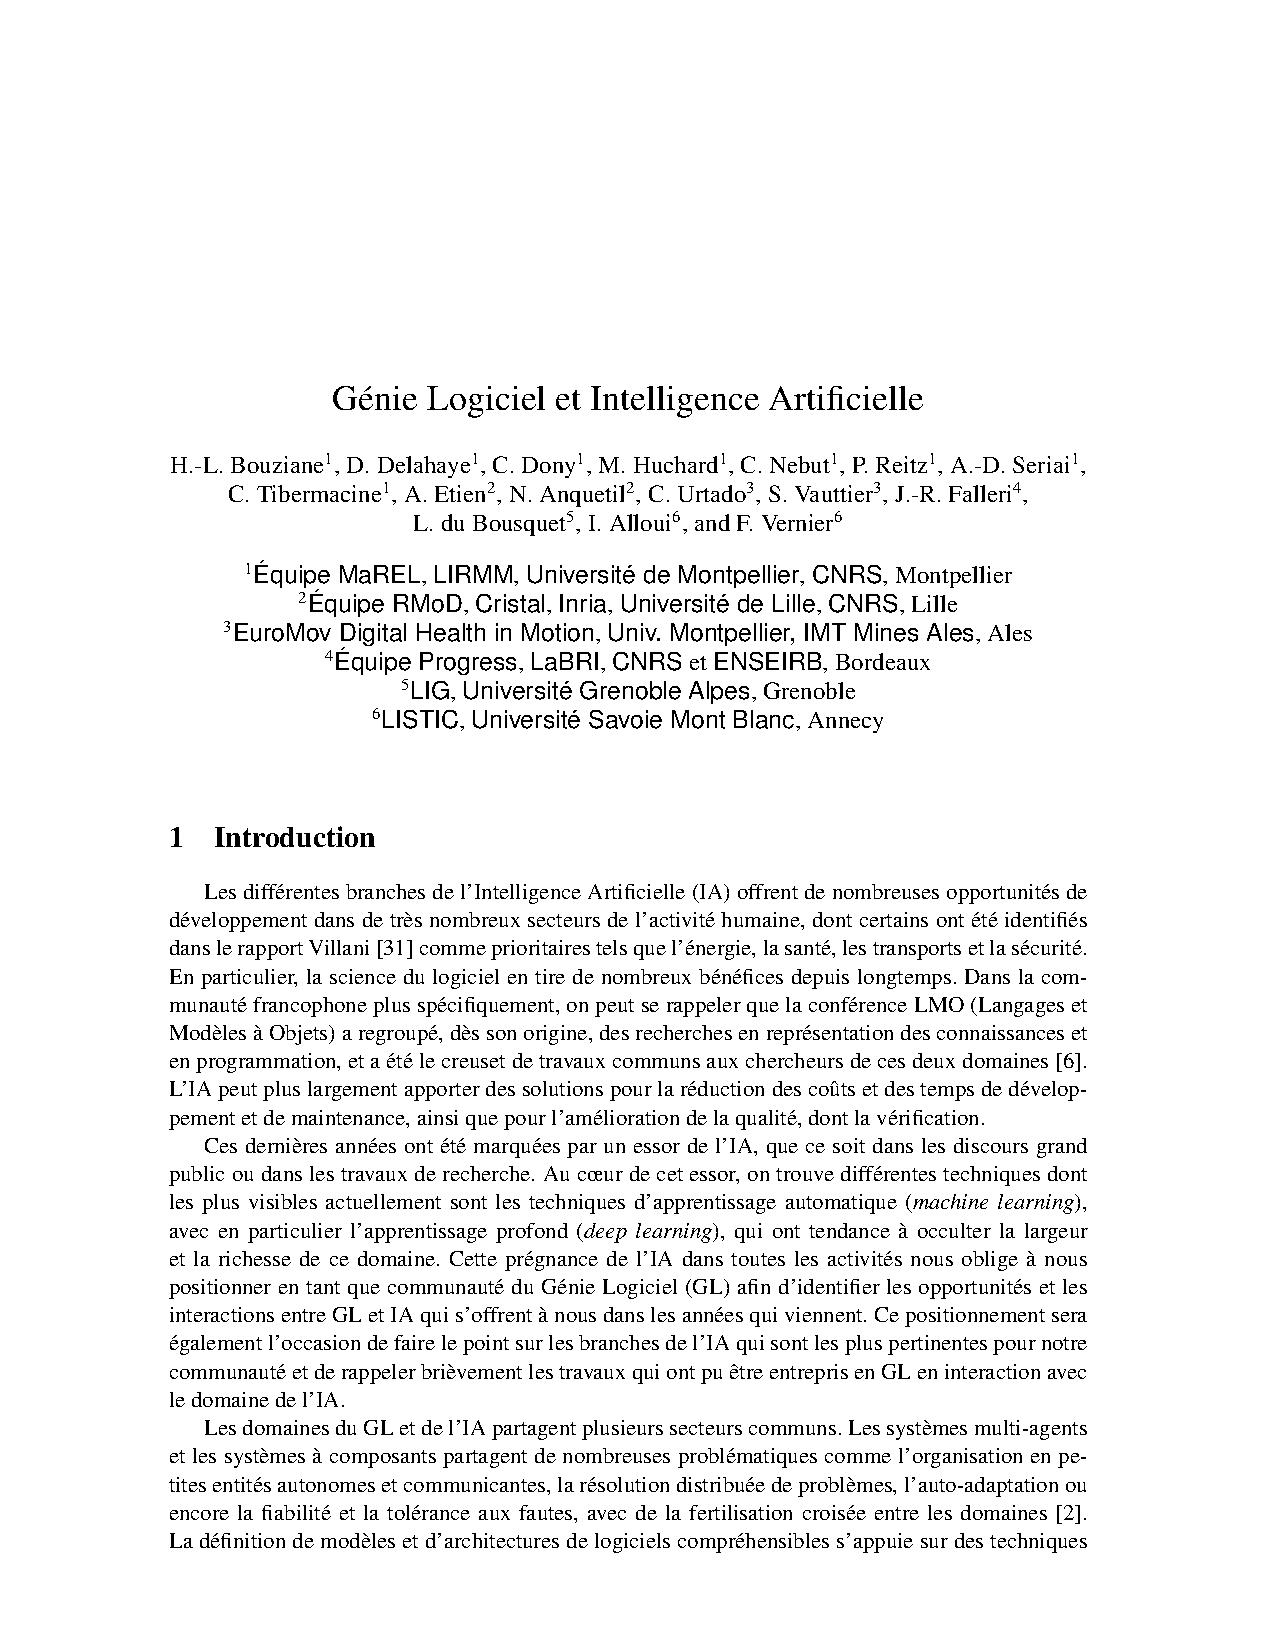
\includepdf[pages=-,pagecommand={\thispagestyle{plain}}]{Defis/Intelligence_Artificielle.pdf}

\label{debuggers}
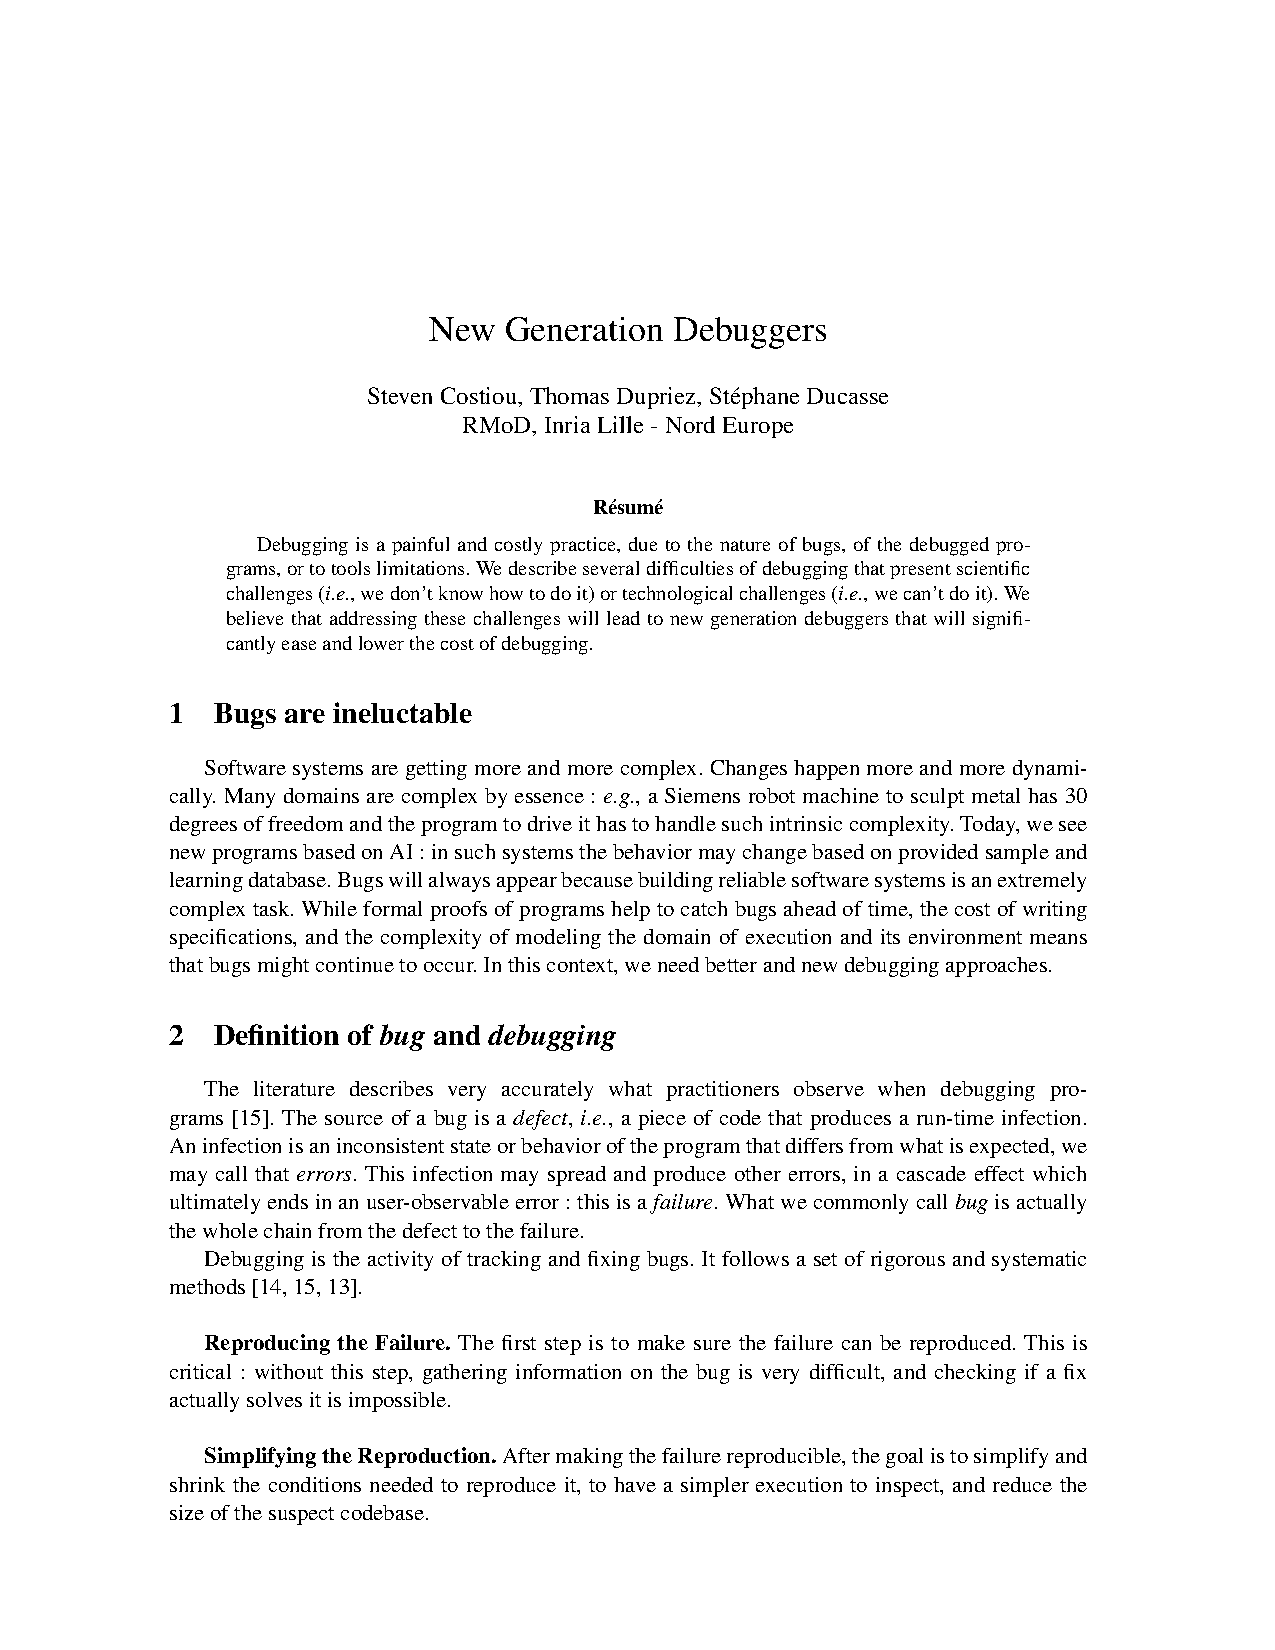
\includepdf[pages=-,pagecommand={\thispagestyle{plain}}]{Defis/New_Generation_Debuggers.pdf}


\label{reconfiguration}
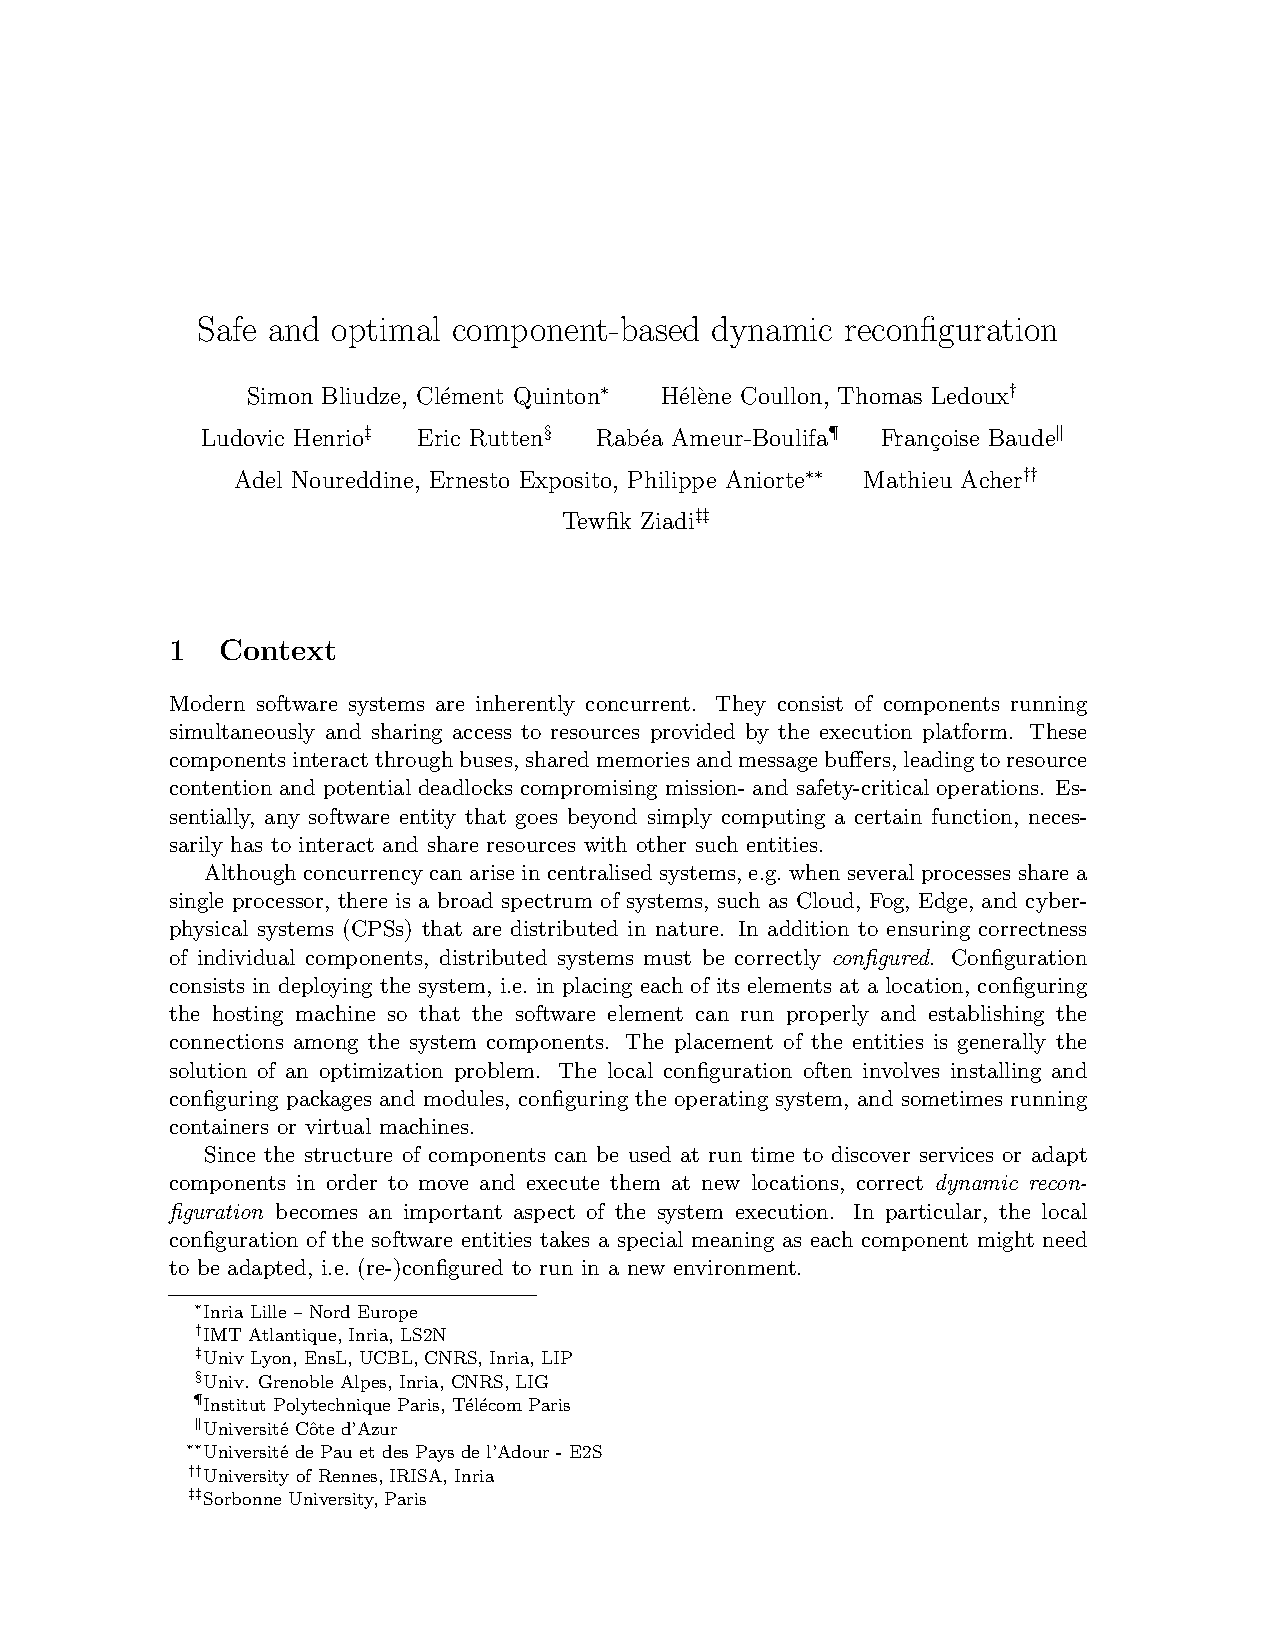
\includepdf[pages=-,pagecommand={\thispagestyle{plain}}]{Defis/Safe_and_optimal_component-based dynamic reconfiguration.pdf}

\label{GLE}
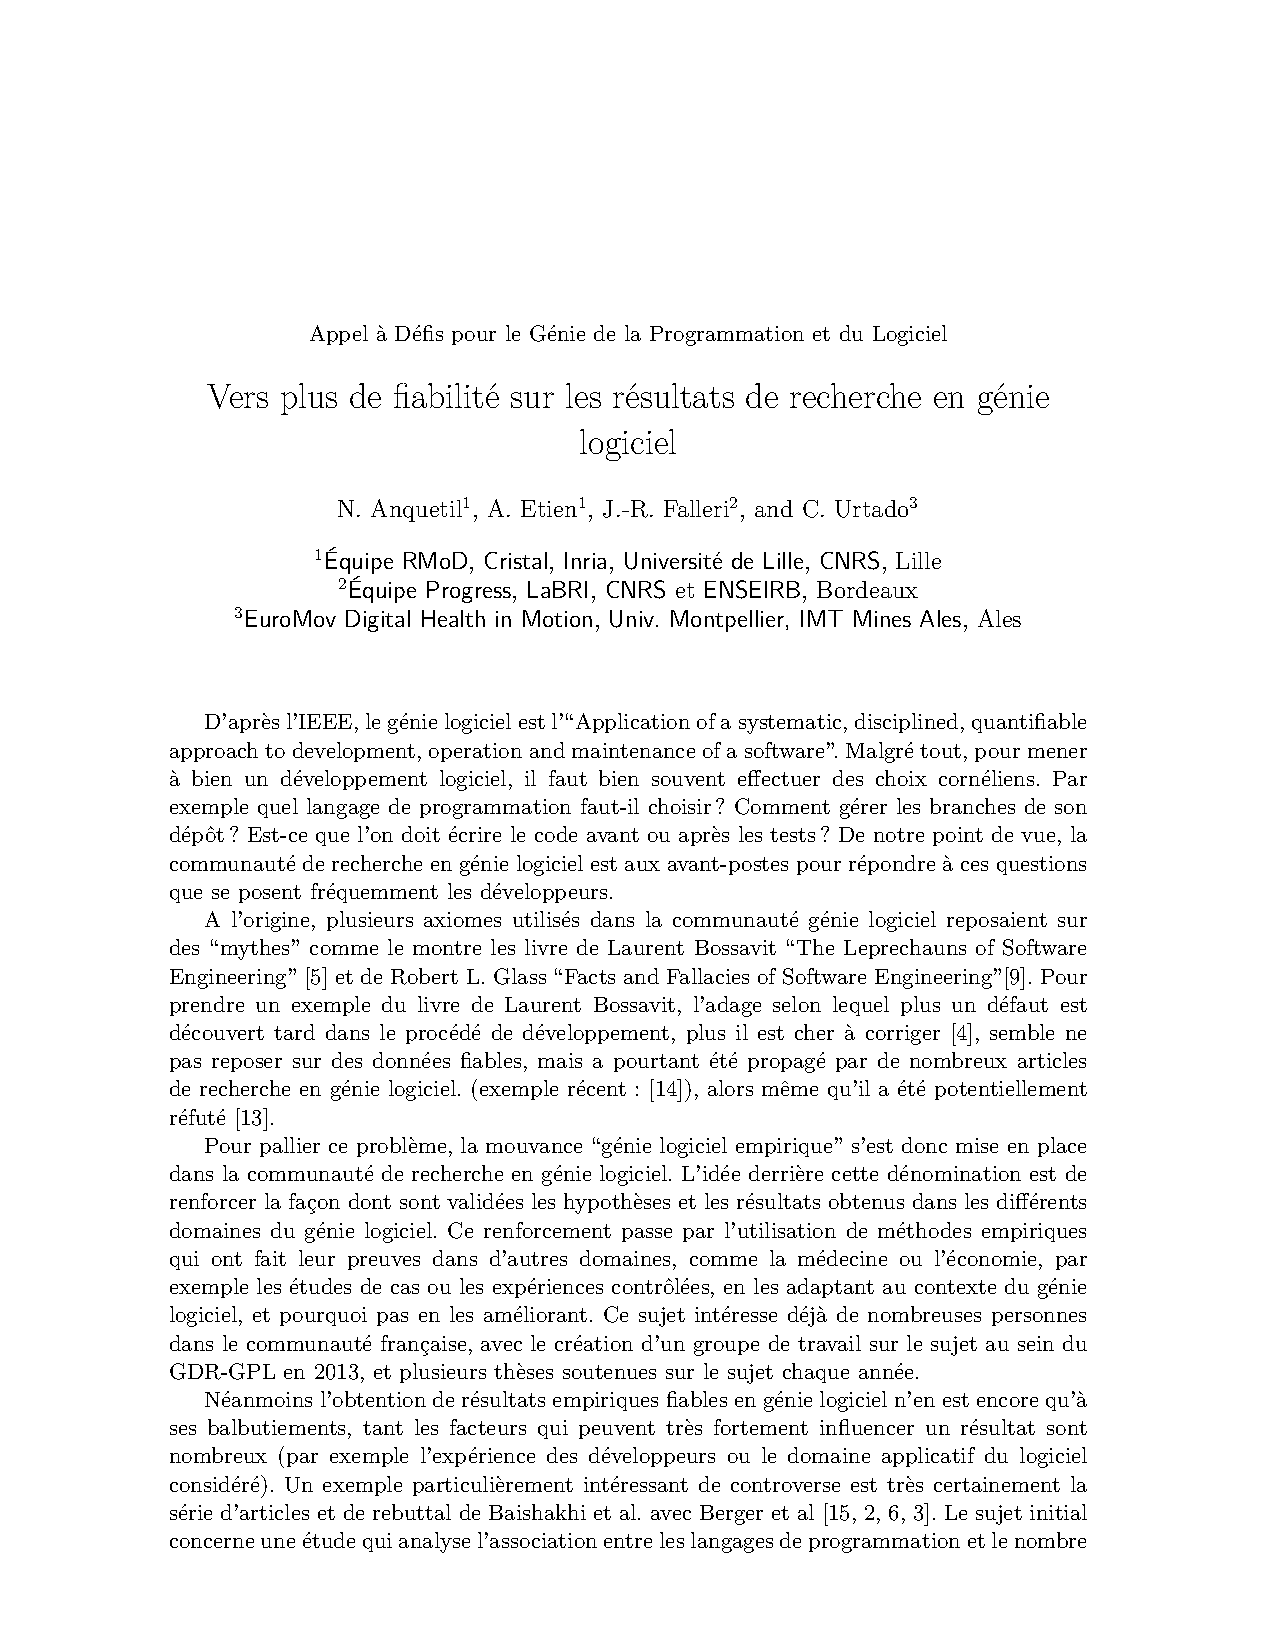
\includepdf[pages=-,pagecommand={\thispagestyle{plain}}]{Defis/Vers_plus_de_fiabilite_Res_recherche.pdf}

\label{securite}
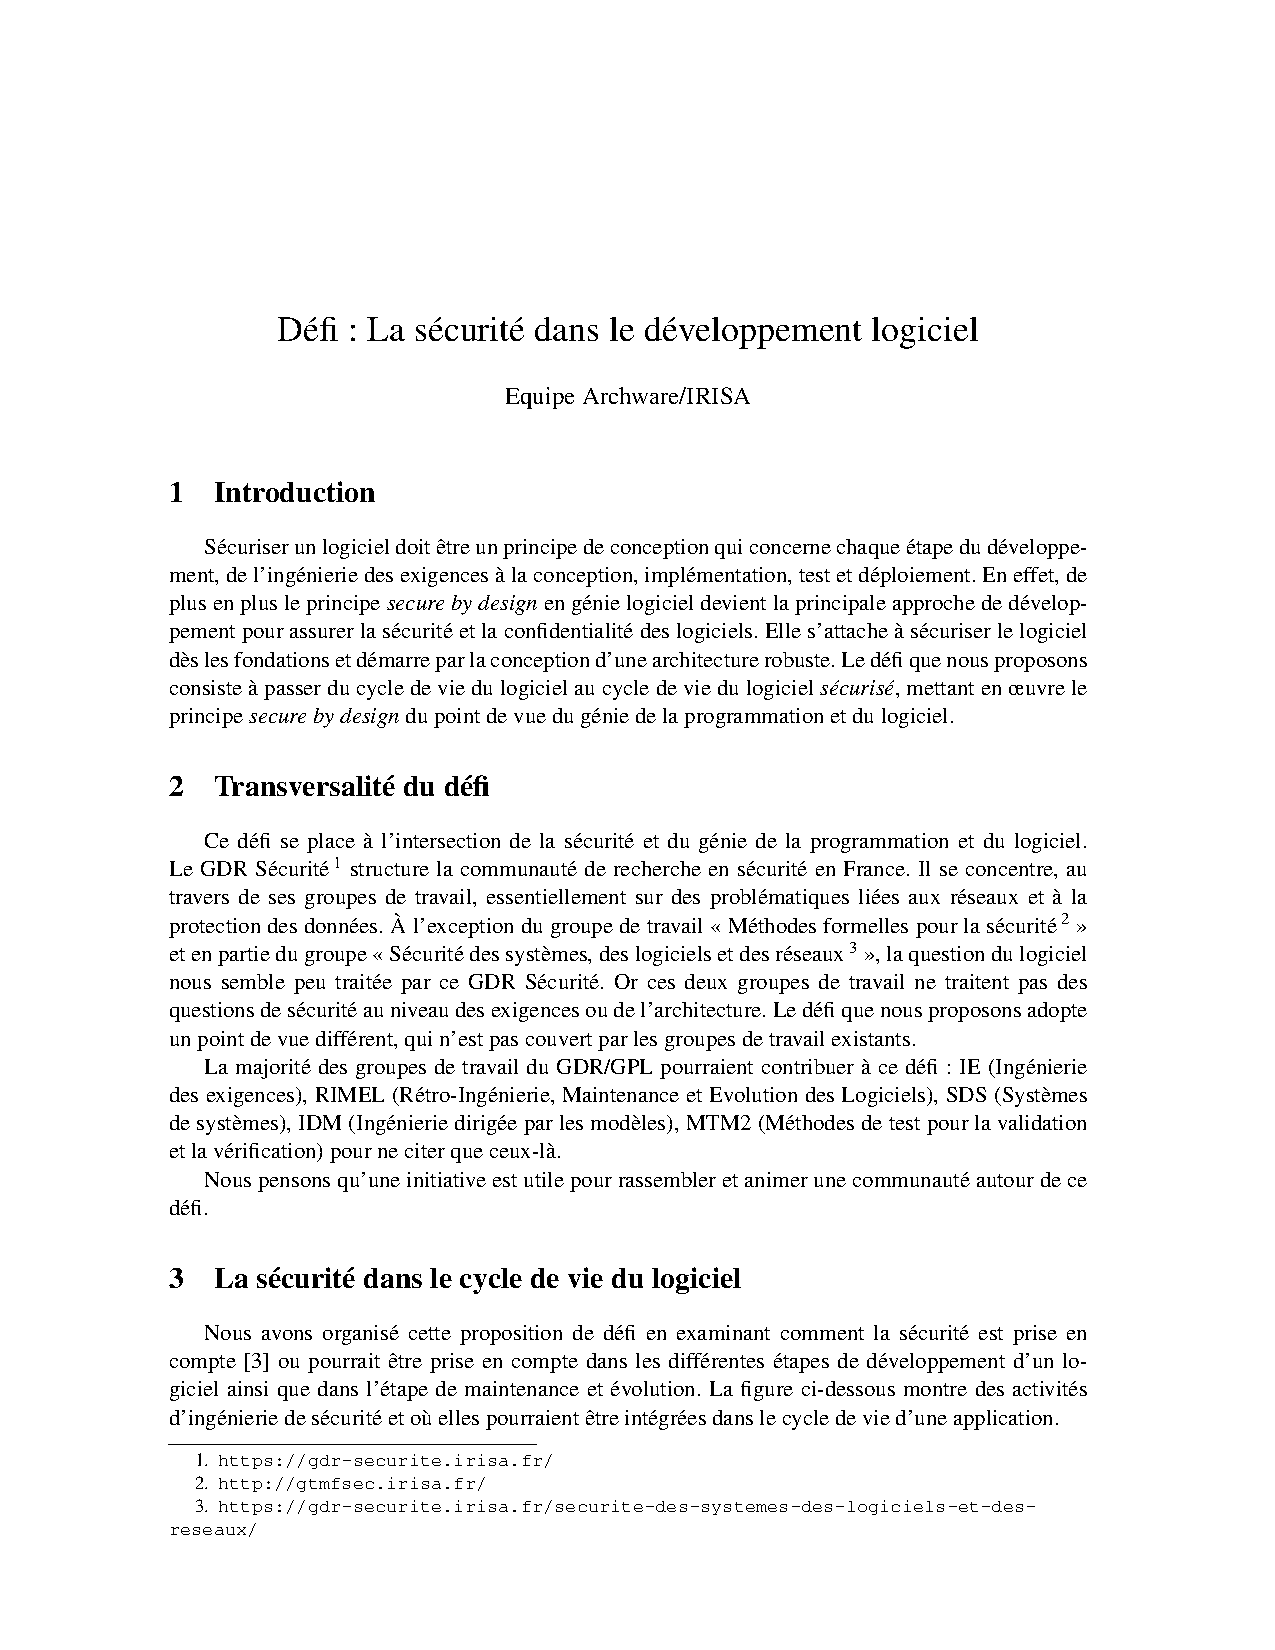
\includepdf[pages=-,pagecommand={\thispagestyle{plain}}]{Defis/securite_dans_le_developpement_logiciel.pdf}

\end{document}
